\section{Introduction}
\label{sec:intro}

The emergence of Large Vision Language Models (LVLMs) has advanced multimodal reasoning by enabling unified understanding of visual and textual modalities \cite{zhu2024minigpt, Liu2024aVisualInstructionTuning, Liu2024bImprovedBaselines, liu2025multimodal}. Trained on large-scale image–text data, these models integrate strong visual perception with rich language knowledge and have shown impressive generalization across various tasks. In medicine, Medical LVLMs (Med-LVLMs) demonstrate promising capabilities in medical visual question answering \cite{Lau2018VQARAD, Zhang2023PMCVQA}, radiology report generation \cite{demner2015preparing, johnson2019mimic}, and multimodal reasoning \cite{Li2023LLaVAMed, Moor2023MedFlamingo}, providing decision support and automated clinical documentation. However, these models still face the challenge of factuality, which mainly arises from modality misalignment between visual and textual streams \cite{Cui2023GPT4VHallucination, zhou2024aligning, zheng2025mllms}. Medical images contain subtle lesion features and imbalanced supervision across modalities, often leading Med-LVLMs to rely on textual priors instead of lesion-grounded evidence, resulting in hallucinated or clinically inconsistent responses \cite{Royer2024MultiMedEval}.

\begin{figure}[!tbp]
    \centering
    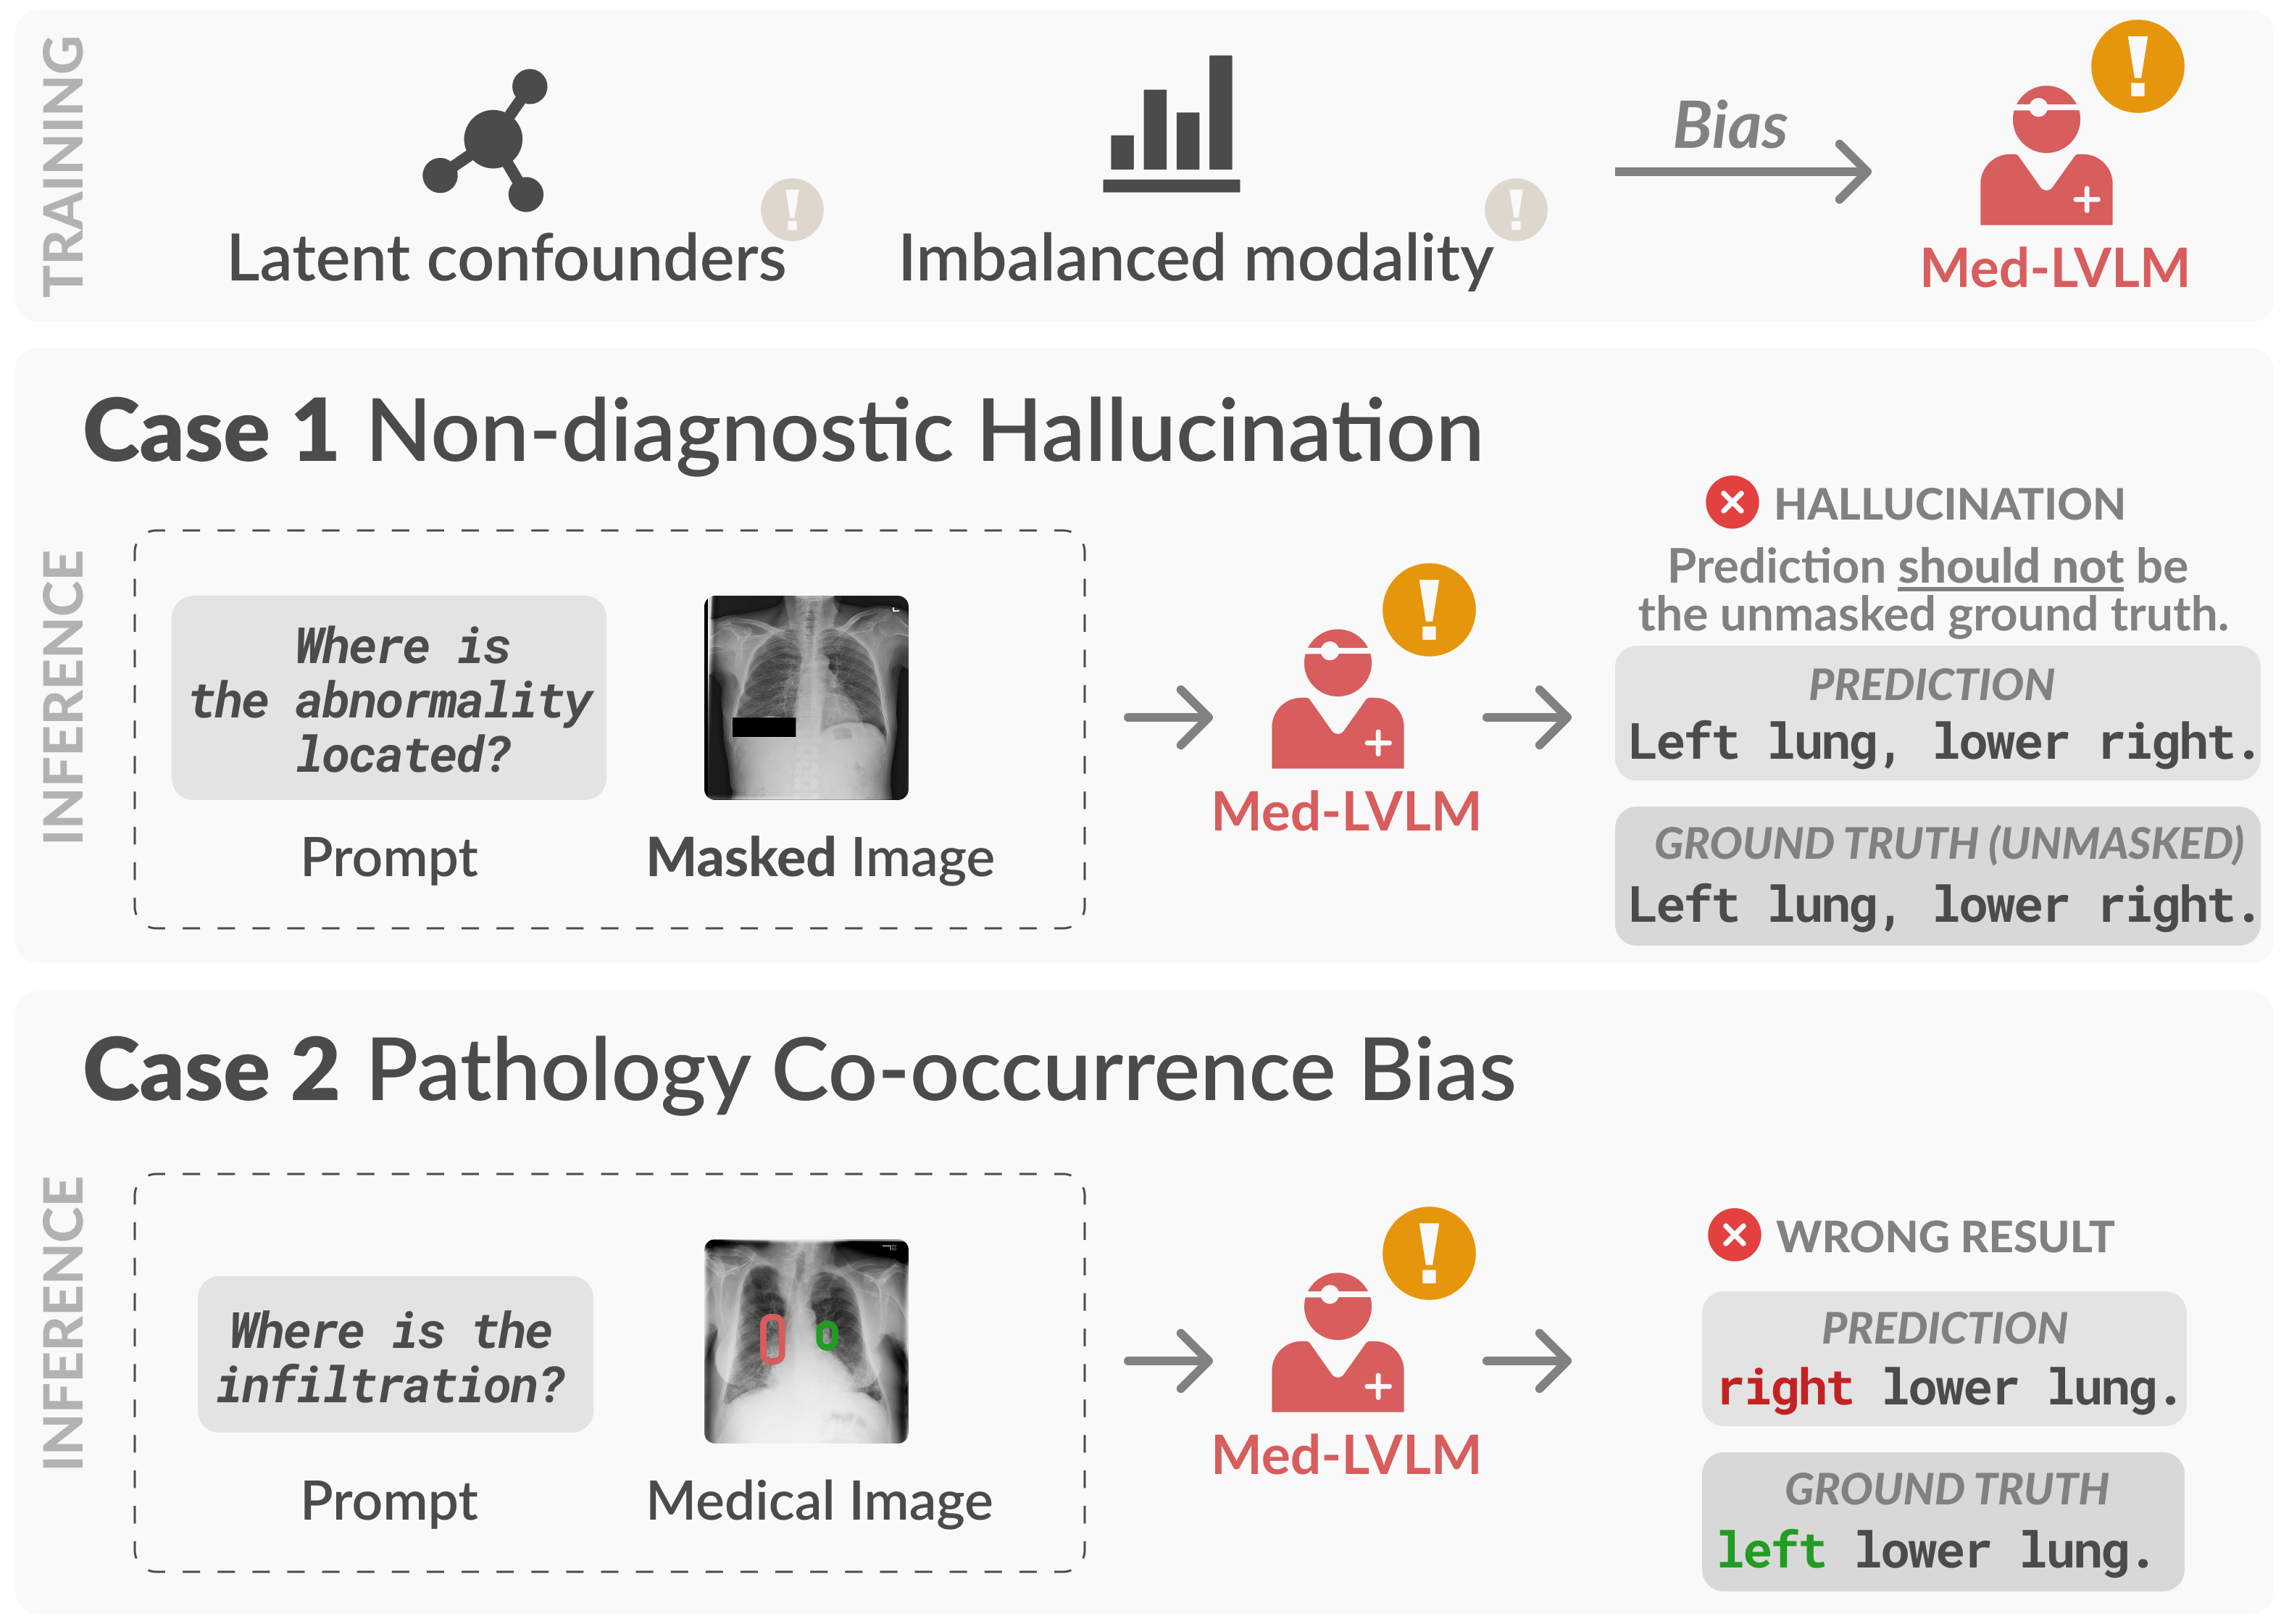
\includegraphics[width=0.5\textwidth]{figs/cvpr_fig1.png}
    \caption{
    % Illustration of how spurious causation affects model inference. 
    Effects of spurious causation on inference.
    (a) Unexpectedly correct predictions given background image. (b) Co-occurrence of multiple pathologies affects the location prediction.}
    \label{fig:intro}
    \vspace{-10pt}
\end{figure}

To address the factuality problem, recent works have introduced preference optimization to improve alignment between visual and textual modalities in Med-LVLMs. These methods fine-tune models by learning from pairwise preferences between clinically relevant and irrelevant responses, aiming to enhance factual grounding and reduce hallucinations. However, most existing approaches simply leverage the preference data generation process originally designed for aligning general LVLMs on natural images \cite{rafailov2023direct, Bai2022RLHF, zhou2024aligning}. Directly transferring such pipelines to the medical domain neglects the unique characteristics of clinical data, where diagnostic correctness and lesion localization are essential. A recent study has highlighted the importance of clinical relevance in constructing effective preference data, proposing to evaluate and weight samples according to medical significance \cite{Zhu2025MMedPO}. Nevertheless, these approaches still rely heavily on statistical associations between textual cues and disease labels, overlooking the influence of spurious causation that arises from biased modality interactions. As a result, even optimized models may continue to depend on spurious correlations rather than true lesion-grounded reasoning, limiting their factuality in clinical scenarios.

In medical reasoning, reliability depends strongly on the model’s ability to generate clinically consistent rationales rather than superficial correlations. However, existing Med-LVLMs often suffer from spurious causation, where predictions are influenced by latent confounders or imbalanced modality signals. One major cause arises from biased statistical associations, in which background regions or contextual patterns become spuriously linked to specific diseases. As illustrated in Fig. \ref{fig:intro}(a), even when an image contains only non-diagnostic background, the model can still predict the correct disease label, indicating an over-reliance on contextual priors instead of lesion evidence. Another common source of spurious effect is pathology co-occurrence bias, where correlated abnormalities lead the model to exploit coincidental features during learning. For example, as shown in Fig. \ref{fig:intro}(b), when pleural effusion and infiltration frequently appear together, the model tends to associate infiltration features with pleural effusion because the training data contain substantially more cases of infiltration in the lower right lung and both conditions exhibit overlapping visual patterns. These observations highlight that mitigating spurious modality dependencies is essential for improving the factual reliability of Med-LVLMs in clinical reasoning.

A principled way to mitigate such spurious causation is to conduct a randomized controlled trial, collecting multimodal clinical data under diverse combinations of lesion and background conditions. In theory, such balanced sampling can disentangle visual evidence from contextual bias and reveal the true causal effect of lesion features on diagnostic outcomes \cite{Thirunavukarasu2023LLMInMedicine}. However, this approach is infeasible in practice because it requires extensive manual annotation and controlled patient recruitment. Recent work such as MMedPO \cite{Zhu2025MMedPO} partially addresses this issue by introducing local noise to lesion areas, which can be interpreted as an intervention on biased training distributions. Yet, this strategy remains sub-optimal since it fails to decouple beneficial background–lesion interactions from harmful ones. In real clinical images, background cues such as tissue density, lung boundary, or rib contrast often provide useful priors when jointly considered with lesion morphology \cite{Royer2024MultiMedEval, Cui2023GPT4VHallucination}. For example, distinguishing pleural effusion from lower-lobe infiltration depends not only on lesion opacity but also on surrounding pleural line continuity and diaphragm curvature \cite{yamada2024pictorial}. Therefore, an effective debiasing framework should preserve clinically meaningful lesion–background relationships while removing confounding dependencies that distort modality alignment.

To address the above challenge, we propose a \textbf{Ca}usal \textbf{Med}ical \textbf{P}reference \textbf{O}ptimization framework (\textbf{CaMedPO}), which mitigates spurious causation while preserving the valuable indirect effect between lesion and background features. CaMedPO can be seamlessly integrated with existing DPO-based alignment methods to further enhance the performance of Med-LVLMs, serving as a general and model-agnostic optimization paradigm. Specifically, we formulate a causal graph that connects multimodal inputs to the reward function, enabling theoretical analysis of how biased reference policies influence downstream alignment. Based on this formulation, CaMedPO derives a principled objective that improves robustness even when the SFT-based reference model is biased. Within this causal structure, we explicitly decouple the harmful direct effect, which transmits bias from shortcut correlations, and the valuable indirect effect, which captures the clinically meaningful joint influence of lesion and contextual cues on diagnostic reasoning. During preference construction, we build factual and counterfactual outcome pairs by employing a lesion detection model to identify clinically relevant regions, which are then used to form paired samples for causal effect estimation. The factual outcomes preserve the normal lesion–background association, while the counterfactual ones intervene on lesion evidence to isolate indirect effects. In the inference phase, the model is trained on normal preference pairs, ensuring consistency with standard alignment while benefiting from causal debiasing during optimization. In summary, our main contributions are threefold:

\noindent $\bullet$ We introduce a causal framework to analyze how biased reference policies propagate harmful direct effects in medical vision–language alignment. This formulation reveals that factuality degradation originates from spurious causation within modality interactions.

\noindent$\bullet$ We propose CaMedPO, a model-agnostic debiasing approach that mitigates spurious causal effects while preserving the valuable indirect effect between lesion and background features. CaMedPO constructs factual–counterfactual outcome pairs based on lesion detection and can be seamlessly integrated with existing DPO methods to enhance robustness.

\noindent$\bullet$ Extensive experiments on Med-VQA and medical report generation benchmarks demonstrate that CaMedPO consistently improves factual accuracy and clinical relevance across multiple Med-LVLMs, highlighting its broad applicability and effectiveness in trustworthy multimodal medical reasoning.